% Created 2024-04-12 Fri 16:55
% Intended LaTeX compiler: pdflatex
\documentclass[10pt,table,dvipsnames,compress]{beamer}
\usepackage[utf8]{inputenc}
\usepackage[T1]{fontenc}
\usepackage{graphicx}
\usepackage{longtable}
\usepackage{wrapfig}
\usepackage{rotating}
\usepackage[normalem]{ulem}
\usepackage{amsmath}
\usepackage{amssymb}
\usepackage{capt-of}
\usepackage{hyperref}
\usetheme{default}
\useinnertheme{rounded}
\useoutertheme[subsection=false]{miniframes}
\date{}
\title{MELANOBS: forest cover change, carbon, and biodiversity data in Melanesia}
\title[MELANOBS]{MELANOBS: forest cover change, carbon, and biodiversity data in Melanesia}
\usepackage{lmodern}
\usepackage{pgf}
\usepackage{color}
\usepackage[english,french]{babel}
\definecolor{vertmoyen}{RGB}{51,110,23} % vert moyen
\definecolor{blueFRB}{HTML}{31859c}
\usecolortheme[named=blueFRB]{structure}
\usepackage{tabularx} % varier la largeur du tableau
\usepackage{layout}
\setlength{\LTleft}{-5cm plus 1 fill}
\setlength{\LTright}{-5cm plus 1 fill}
\usepackage{booktabs}
\usepackage{arydshln} %% dashlines for tabular
\newcommand{\logit}{\text{logit}}
\newcommand{\bs}[1]{\boldsymbol{#1}}
\newcommand{\R}{\textnormal{\sffamily\bfseries R}}
\newcommand{\pkg}[1]{{\fontseries{b}\selectfont #1}}
\newcolumntype{C}[1]{>{\centering\arraybackslash}m{#1}}

\setbeamertemplate{footline}[frame number]
\setbeamertemplate{frametitle}{%
\usebeamerfont{frametitle}\insertframetitle%
\vphantom{g} % To avoid fluctuations per frame
\par
\centering 
\includegraphics[width=\textwidth]{figs/Barre_couleur}
}
\beamertemplatenavigationsymbolsempty

% Logo
\newif\ifplacelogo % create a new conditional
\logo{\ifplacelogo
\includegraphics[width=0.6\textwidth]{figs/partners_logos}\fi}

%Call table of contents at the beginning of each section
\AtBeginSection[]{
\placelogotrue
\begin{frame}
\frametitle{Plan}
\begin{columns}[c]
\begin{column}{0.5\textwidth}
\tableofcontents[sections=1,currentsection]
\vspace{0.5cm}
\tableofcontents[sections=2,currentsection]
\end{column}
\begin{column}{0.5\textwidth}
\tableofcontents[sections=3,currentsection]
\vspace{0.5cm}
\tableofcontents[sections=4,currentsection]
\end{column}
\end{columns}
\end{frame}
\placelogofalse
}

\AtBeginSubsection[]{}

\hypersetup{
colorlinks=true,
linkcolor=Black,
filecolor=Maroon,
citecolor=Blue,
urlcolor=Maroon}

% Disable monospaced font for URLs
\urlstyle{same}

\hypersetup{
 pdfauthor={Ghislain Vieilledent},
 pdftitle={MELANOBS: forest cover change, carbon, and biodiversity data in Melanesia},
 pdfkeywords={},
 pdfsubject={},
 pdfcreator={Emacs 29.2 (Org mode 9.6.15)}, 
 pdflang={English}}
\begin{document}


% {
%   % Use background image
%   \usebackgroundtemplate{%
%     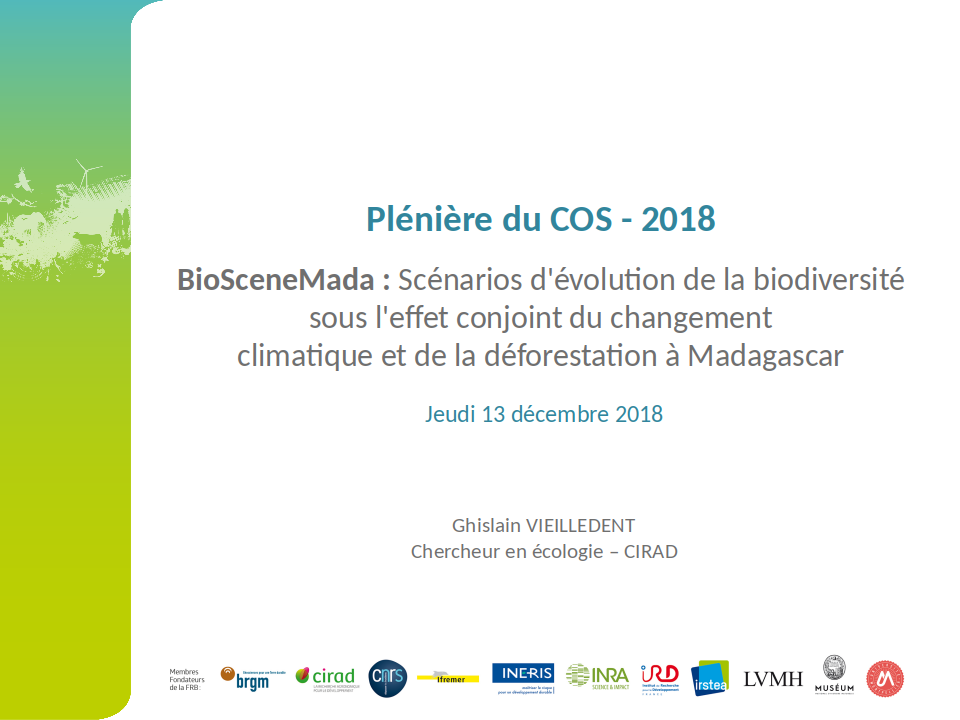
\includegraphics[height=\paperheight,width=\paperwidth]{figs/Masque.png}
%   }
%   \setbeamertemplate{navigation symbols}{}
%   % Remove shadow from block
%   \setbeamertemplate{blocks}[rounded][shadow=false]
%   \begin{frame}[plain]
%   \end{frame}
% }

% Title page
{
  \setbeamertemplate{navigation symbols}{}
  \begin{frame}[plain, noframenumbering]
  \begin{center}
  \small{\textbf{MELANOBS workshop -- Noumea, April 2024}}
  \end{center}
  \vspace{-0.5cm}
  \titlepage % Presentation first page
  \vspace{-3cm}
  \begin{center}
    
\includegraphics[width=\textwidth]{figs/Barre_couleur}
    
    \vspace{0.25cm}
    
    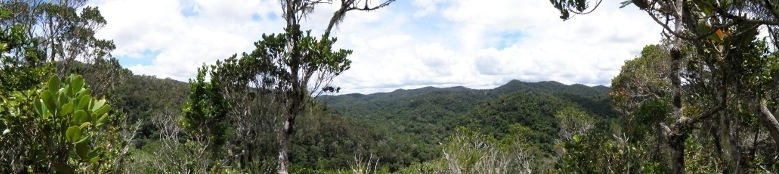
\includegraphics[width=10cm]{figs/Banniere}
    
    \small{Ghislain VIEILLEDENT$^{1}$\hspace{0.25cm}Philippe BIRNBAUM$^{1}$\\
      \vspace{0.10cm}David BRUY$^{2}$\hspace{0.25cm}Thomas IBANEZ$^{2}$}
      
    \vspace{0.25cm}
    
    {\scriptsize
      \begin{tabular}{l}
        $[1]$ \textbf{Cirad} UMR AMAP, $[2]$ \textbf{IRD} UMR AMAP
      \end{tabular}
    }
    
    
\includegraphics[width=0.8\textwidth]{figs/partners_logos}
    
  \end{center}
  \end{frame}
}

% %%%%%%%%%%%%%%%%%%%%%%%%%%%%%%%%%%%%%%%%%%%%%%%%%%%%%%%%%%%%%%%%

\placelogotrue
\begin{frame}
  \frametitle{Outline}
  \begin{columns}[c]
    \begin{column}{0.5\textwidth}
      \tableofcontents[sections=1]
      \vspace{0.5cm}
      \tableofcontents[sections=2]
    \end{column}
    \begin{column}{0.5\textwidth}
        \tableofcontents[sections=3]
        \vspace{0.5cm}
        \tableofcontents[sections=4]
    \end{column}
  \end{columns}
\end{frame}
\placelogofalse

\section{Introduction}
\label{sec:org69353f7}

\subsection{Context}
\label{sec:org52c8df6}

\begin{frame}[label={sec:orga7999bc}]{Context}
\begin{center}
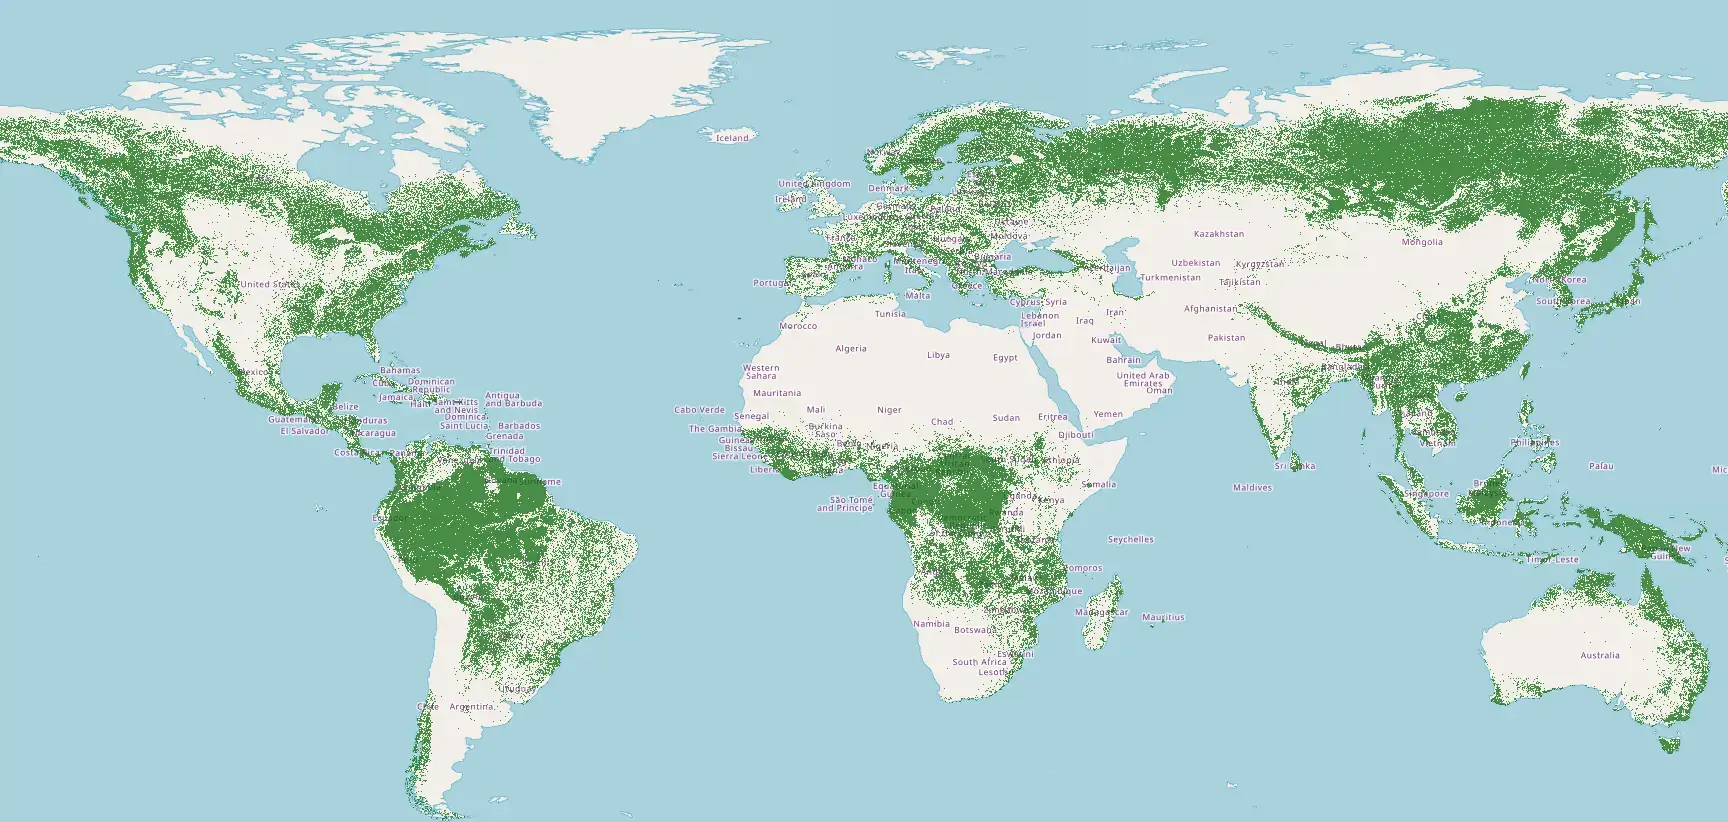
\includegraphics[width=8cm]{figs/forest_cover_jrc_2020.png}
\end{center}

\begin{itemize}
\item Tropical forests: 50\% of terrestrial biodiversity.
\item Tropical deforestation: 15\% of anthropogenic carbon emissions.
\item Mapping forest cover, carbon stocks and biodiversity is essential for conservation planning.
\end{itemize}
\end{frame}

\begin{frame}[label={sec:orge9de18c}]{Objectives}
\begin{center}
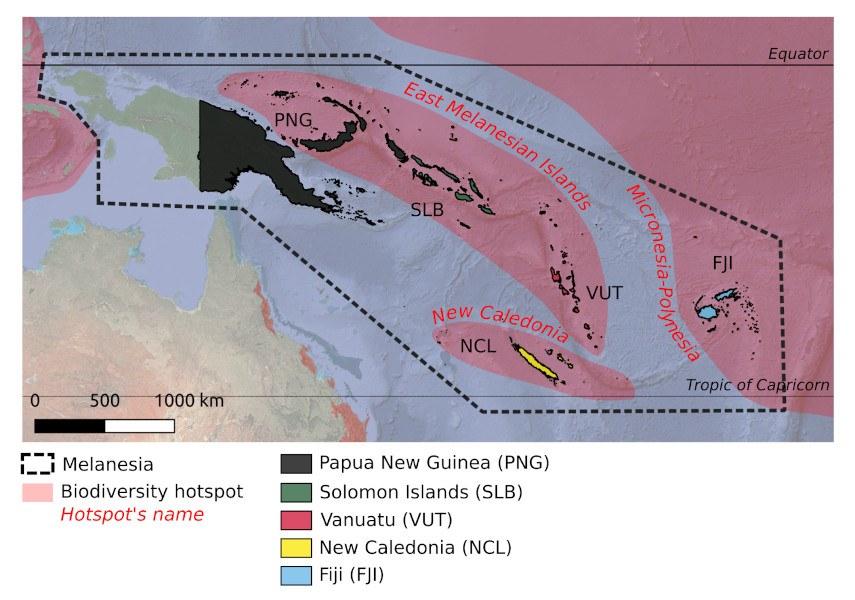
\includegraphics[width=8cm]{figs/carte_melanobs.jpg}
\end{center}

\begin{itemize}
\item MELANOBS: building a Melanesian forest observatory.
\item Which data on forest cover, carbon stock and biodiversity is available for Melanesian countries?
\end{itemize}
\end{frame}

\section{Forest cover change data}
\label{sec:org0d5eb83}

\subsection{FAO FRA estimates}
\label{sec:org380aac1}

\begin{frame}[label={sec:org56e2a78}]{FAO FRA estimates, forest cover}
\textbf{Forest cover estimates (in Kha).}

\begin{center}
\begin{tabular}{lrrrr}
Source & FRA 2015 & prim. forest & GFC30 2020 & TMF 2020\\[0pt]
\hline
PNG & 36024 & 27200 & 39000 & 39304\\[0pt]
Salomon Islands & 2527 & 1738 & 2350 & 2739\\[0pt]
Vanuatu & 442 & 205 & 986 & 1152\\[0pt]
Fiji & 1107 & 0 & 1050 & NA\\[0pt]
New Caledonia & 839 & 338 & 1150 & 855\\[0pt]
\end{tabular}
\end{center}

\begin{itemize}
\item Forest Ressources Assessment (FRA) from the Food and Agriculture Organization (FAO).
\item Estimates are reported by countries to FAO.
\item Not frequently updated.
\item There is no map of forest cover change provided by FAO.
\end{itemize}
\end{frame}

\begin{frame}[label={sec:org0e2700e}]{FAO FRA estimates, gross deforestation}
\textbf{Mean annual deforestation (in ha).}

\begin{center}
\begin{tabular}{lrrr}
Source & FRA & GFC30 & TMF\\[0pt]
 & 2015--2020 & 2010--2020 & 2010--2020\\[0pt]
\hline
PNG & 34000 & 104678 & 48691\\[0pt]
Salomon Islands &  & 13460 & 1751\\[0pt]
Vanuatu &  & 939 & 564\\[0pt]
Fiji &  & 2663 & NA\\[0pt]
New Caledonia &  & 1328 & 2425\\[0pt]
\end{tabular}
\end{center}

\begin{itemize}
\item Rather good estimates of forest cover but poor estimates of deforestation/regrowth.
\item Differentiate forest types: forest, primary forest, plantations
\end{itemize}
\end{frame}

\subsection{Global datasets}
\label{sec:org20d92bf}

\begin{frame}[label={sec:org4e46164}]{Global Forest Change (GFC)}
\begin{center}
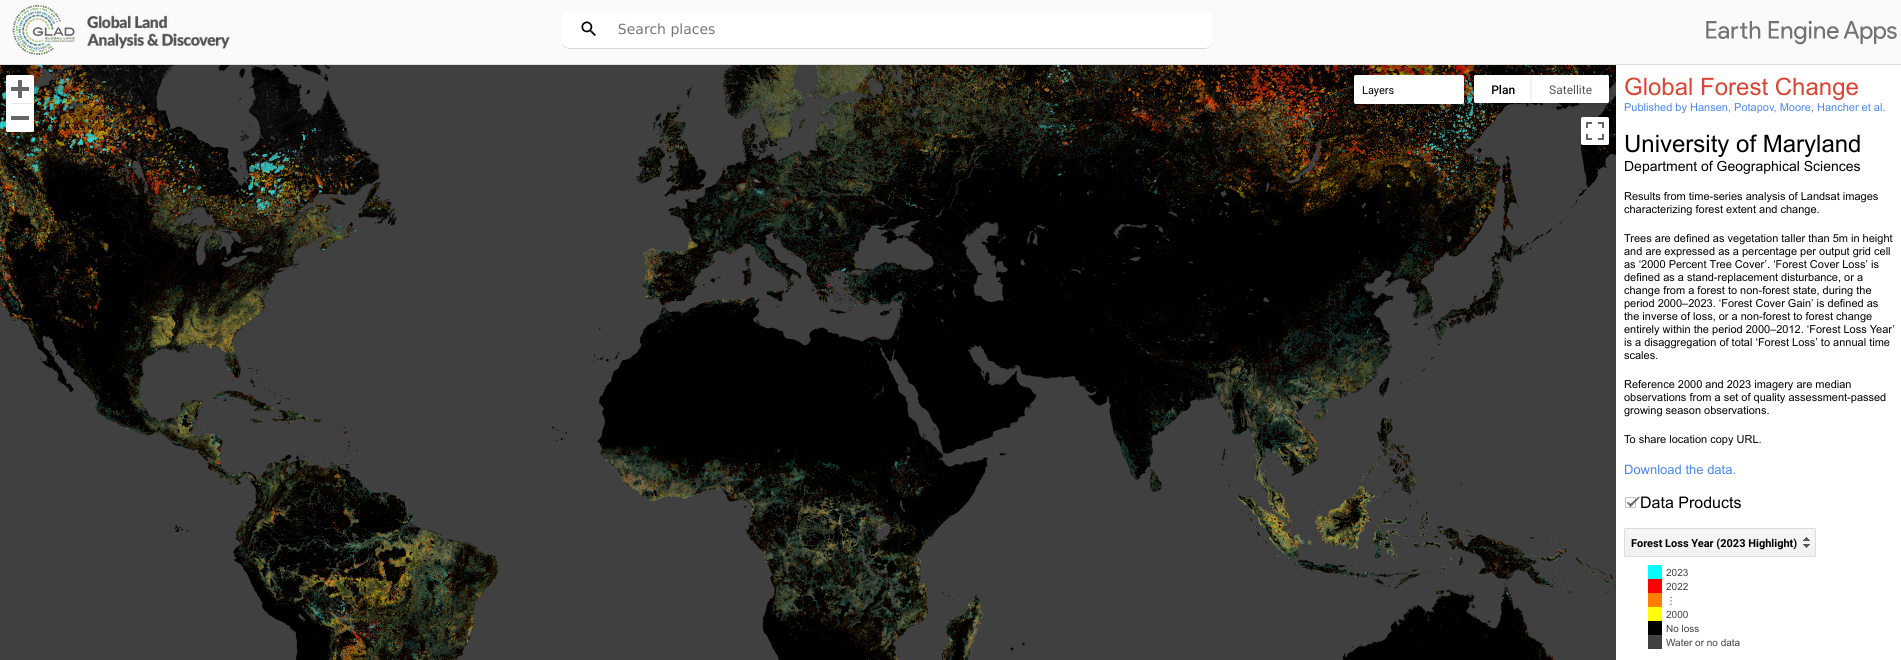
\includegraphics[width=8cm]{figs/fcc/gfc.png}
\end{center}

\begin{itemize}
\item \href{https://glad.earthengine.app/view/global-forest-change}{Global Forest Change} (Hansen et al. 2013, Univ. of Maryland).
\item Used by \href{https://www.globalforestwatch.org/}{Global Forest Watch} (GFW): platform about the world forests. GFW releases the \href{https://research.wri.org/gfr/global-forest-review}{Global Forest Review}.
\item It is in fact a tree cover change product. User must define a tree cover threshold to define the forest (e.g. 30\%).
\item Derive from Landsat images from 2000. 30m resolution. One mosaic per year.
\item Largely overestimate forest cover if low tree cover threshold (e.g. 30\%).
\item Underestimate small-scale deforestation (shifting agriculture, logging).
\end{itemize}
\end{frame}

\begin{frame}[label={sec:org5042f65}]{Tropical Moist Forests (TMF)}
\begin{center}
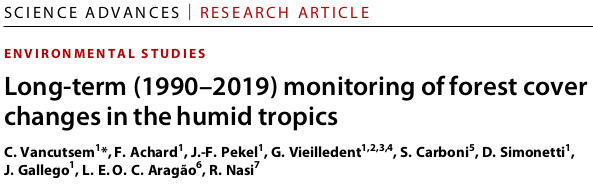
\includegraphics[width=8cm]{figs/fcc/Vancutsem2021.png}
\end{center}

\begin{itemize}
\item \href{https://forobs.jrc.ec.europa.eu/TMF}{Tropical Moist Forests} (Vancutsem et al. 2021, from Joint Research Center).
\item Only consider evergreen tropical forests (tropical moist forests, mangroves, evergreen dry tropical forests). Cannot be used to monitor deciduous dry forests.
\item Derive from Landsat images from 1990. 30m resolution. Time-series at the pixel scale.
\item Fiji is not entirely available (beyond the 180th meridian).
\item Overestimate forest cover in some areas (e.g. Vanuatu, Mare island in New Caledonia).
\end{itemize}
\end{frame}

\subsection{National data}
\label{sec:org4156c30}

\begin{frame}[label={sec:org5f7b575}]{National data}
\begin{itemize}
\item There is room to improve forest cover change map at the national scale.

\item MELANOBS objectives:
\begin{itemize}
\item State of the forest cover change data available at the national scale.
\item Derive up to date forest cover change maps for participating countries.
\end{itemize}
\end{itemize}
\end{frame}

\begin{frame}[label={sec:orgc285709}]{In New-Caledonia}
\begin{center}
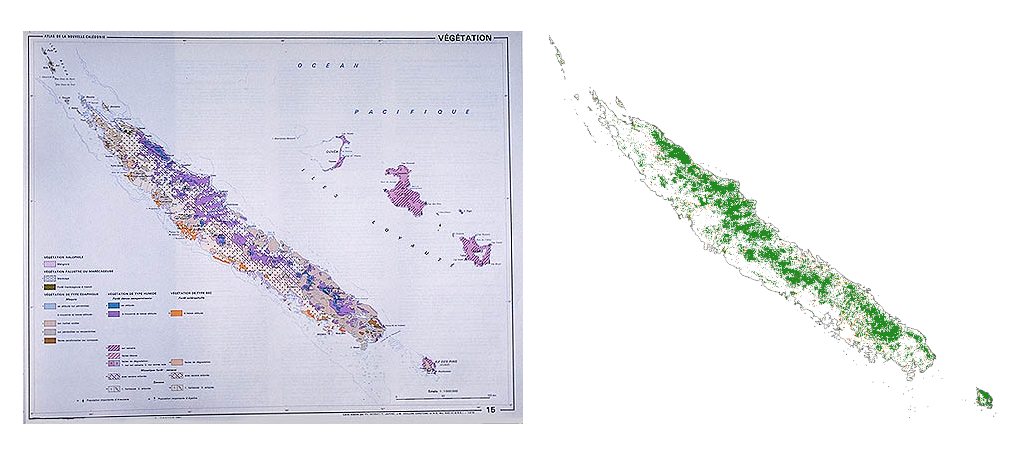
\includegraphics[width=9cm]{figs/fcc/fcc_nc.png}
\end{center}

\begin{itemize}
\item Coarse vegetation maps from IRD (Jaffre, Morat).
\item Forest cover change map for 2000-2010-2020 derived from TMF.
\item Natural forest cover map for year \textasciitilde{}2020 derived from photo-interpretation of aerial images.
\end{itemize}
\end{frame}

\section{Carbon stock data}
\label{sec:orgfad5893}

\subsection{Global data-sets}
\label{sec:org6ed78b0}

\begin{frame}[label={sec:orgf9562a2}]{Global data-sets}
\begin{center}
\footnotesize
\begin{tabular}{lllrl}
Name & Resolution & Reference & Epoch & Method\\[0pt]
\hline
Saatchi & 1 km & Saatchi 2011 & 2000 & GLAS, MODIS, QSCAT, SRTM\\[0pt]
WHRC-Baccini & 500 m & Baccini 2012 & 2008 & GLAS, MODIS, SRTM\\[0pt]
Avitabile & 1 km & Avitabile 2016 & 2008 & fusion of Saatchi and Baccini\\[0pt]
GFW-Baccini & 30 m & Baccini 2017 & 2000 & GLAS, Landsat, SRTM\\[0pt]
CCI Biomass & 100 m & Santoro 2019 & 2020 & ALOS2, PALSAR 2, Sentinel 1\\[0pt]
GEDI & 1 km & Dubayah 2023 & 2020 & LiDAR GEDI 2, ALS\\[0pt]
more\ldots{} &  &  &  & \\[0pt]
\end{tabular}
\end{center}

\begin{itemize}
\item Usually\textsuperscript{\(\star\)} a three step approach: field data, LiDAR, satellite images (optical or radar).
\item \(\star\) somewhat different for the GEDI product.
\end{itemize}
\end{frame}

\begin{frame}[label={sec:orgc5dcf74}]{Disadvantages of global products}
\begin{figure}[htbp]
\centering
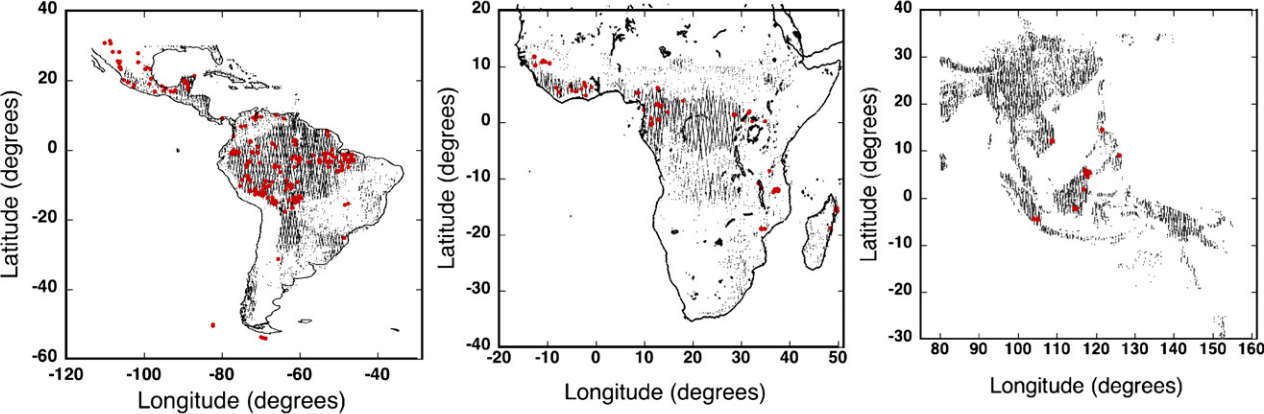
\includegraphics[width=10cm]{figs/carbon/data-saatchi.png}
\caption{\textbf{Field plots used in Saatchi et al. 2011}}
\end{figure}

\begin{itemize}
\item Some countries might be absent from the final map (eg. New Caledonia for Saatchi, WHRC-Baccini and Avitabile).
\item Global models might not be accurate for countries with no field data for calibration.
\item High discrepancies between maps.
\item Resolutions might be coarse: >= 500 m.
\end{itemize}
\end{frame}

\begin{frame}[label={sec:org9edc783}]{GEDI derived AGB map}
\begin{columns}
\begin{column}{0.5\columnwidth}
\begin{center}
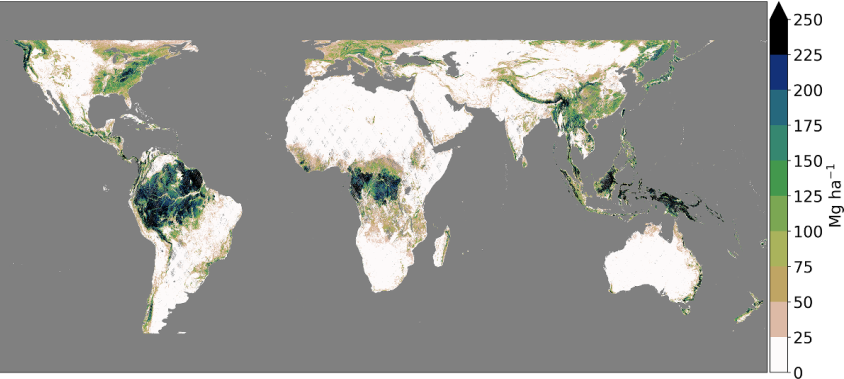
\includegraphics[width=6cm]{figs/carbon/AGB_GEDI.png}
\end{center}
\end{column}

\begin{column}{0.5\columnwidth}
\begin{center}
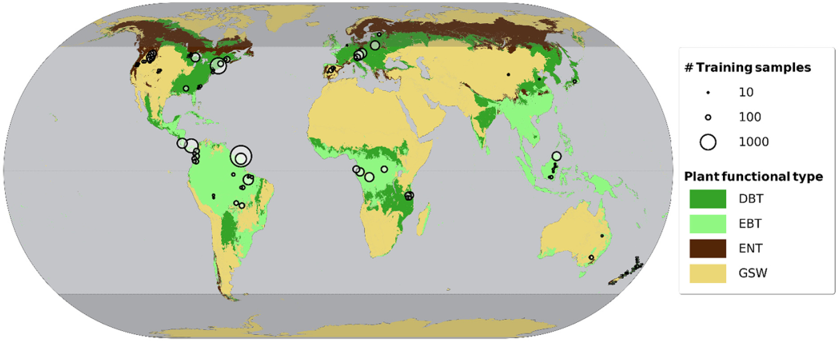
\includegraphics[width=6cm]{figs/carbon/training-data-GEDI.png}
\end{center}
\end{column}
\end{columns}

\begin{block}{}
\begin{itemize}
\item No extrapolation using satellite images and SRTM.
\item GEDI footprints are aggregated within 1 km grid cells.
\item Low resolution: 1 km, location uncertainty of about 25 m.
\item Same problem as for other data-sets: no field data from Melanesia for calibration.
\end{itemize}
\end{block}
\end{frame}

\subsection{National data-sets}
\label{sec:org733fb7a}

\begin{frame}[label={sec:orgc57e625}]{National data-sets}
\end{frame}

\section{Biodiversity data}
\label{sec:orgef5f1e1}

% %%%%%%%%%%%%%%%%%%%%%%%%%%%%%%%%%%%%%%%%%%%%%%%%%%%%%%%%%%

{
  % Use background image
  \usebackgroundtemplate{%
    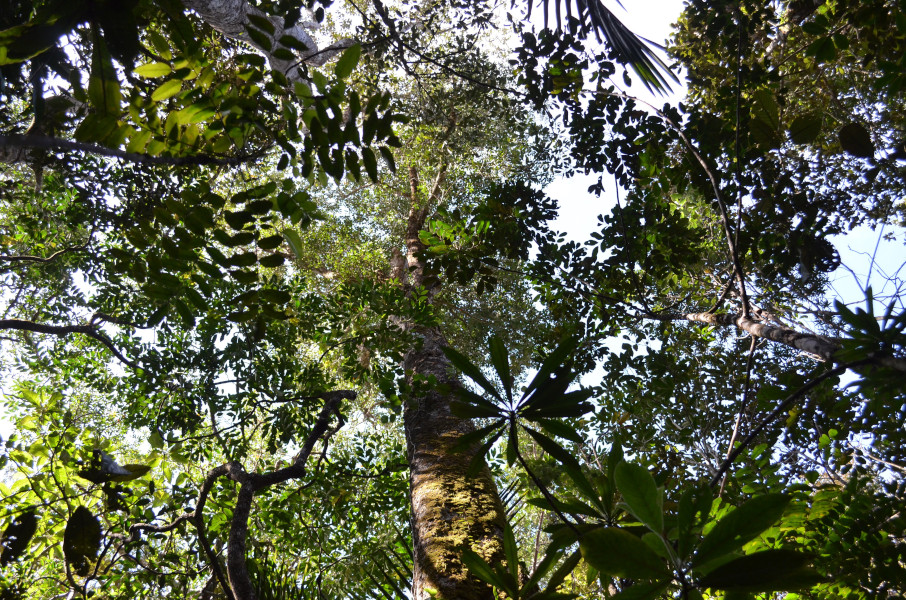
\includegraphics[keepaspectratio=true, height=\paperheight]{figs/Canopy-NC}
  }
  \setbeamertemplate{navigation symbols}{}
  % Remove shadow from block
  \setbeamertemplate{blocks}[rounded][shadow=false]
  \begin{frame}[plain]
  	\vspace*{\stretch{100}} 
    \begin{block}{}
      \begin{center}
        \ldots~Thank you for attention~\ldots \\
        \url{https://ecology.ghislainv.fr/presentations.html} \\
        
\includegraphics[width=0.8\textwidth]{figs/partners_logos}
      \end{center}
    \end{block}
  \end{frame}
}
\end{document}
